\documentclass{article}
\usepackage{textcomp}
\usepackage[utf8x]{inputenc}
\usepackage{graphicx}
\usepackage{xcolor}
\usepackage[most]{tcolorbox}
\usepackage{todonotes}
\usepackage{float}
\usepackage[center]{titlesec}

\begin{document}

  \begin{titlepage}

    \newcommand{\HRule}{\rule{\linewidth}{0.5mm}} % Defines a new command for the horizontal lines, change thickness here

    \center % Center everything on the page

%----------------------------------------------------------------------------------------
%	HEADING SECTIONS
%----------------------------------------------------------------------------------------

    \textsc{\LARGE Technical University of Moldova}\\[1.5cm]
    \textsc{\Large Special Mathematics}\\[0.5cm] % Major heading such as course name

%----------------------------------------------------------------------------------------
%	TITLE SECTION
%----------------------------------------------------------------------------------------

    \HRule \\[0.4cm]
    { \huge \bfseries Laboratory No.3}\\[0.4cm] % Title of your document
    \HRule \\[1.5cm]

%----------------------------------------------------------------------------------------
%	AUTHOR SECTION
%----------------------------------------------------------------------------------------

    \begin{minipage}{0.4\textwidth}
      \begin{flushleft} \large
        \emph{Author:}\\
          st. Polina \textsc{Gore}\\ gr. FAF-161 % Your name
      \end{flushleft}
    \end{minipage}
~
    \begin{minipage}{0.4\textwidth}
      \begin{flushright} \large
        \emph{Supervisor:} \\
        Victor \textsc{Țurcanu} % Supervisor's Name
      \end{flushright}
    \end{minipage}\\[2cm]

%----------------------------------------------------------------------------------------
%	DATE SECTION
%----------------------------------------------------------------------------------------

    {\large \today}\\[2cm] % Date, change the \today to a set date if you want to be precise

%----------------------------------------------------------------------------------------
%	LOGO SECTION
%----------------------------------------------------------------------------------------
    
\includegraphics[width=7cm]{utm2.png}\\[1cm] % Include a department/university logo - this will require the graphicx package

%----------------------------------------------------------------------------------------

    \vfill % Fill the rest of the page with whitespace

  \end{titlepage}

%----------------------------------------------------------------------------------------
%----------------------------------------------------------------------------------------

  \newpage
  \pagenumbering{arabic}

  % -------------- PROBLEM 1------------------------------------------------------

  \section{Problem No.1}
  Write a program that prints the first 10 most frequently used \textbf{words},
  and the number of times it was mentioned.\\
  \centerline{Ex:}
  \begin{tcbraster}[raster columns=5,raster equal height]
    \begin{tcolorbox}[enhanced jigsaw,
      colback=black!10!white,
      coltext=black,
      center,
      sharp corners,
      colframe=black,
      boxrule=0pt]
      the 352

      a 235

      at 120

      . . .

    \end{tcolorbox}
  \end{tcbraster}

  \vspace{2em}

  \subsection{Solution}
    To process the tweets, we have to extract them from a \emph{json} file.\\
    Then split every tweet into words, but first we better lower the letters.\\
    Now, using the function \underline{FreqDist} from \emph{nltk} module,
    we find the frequency of every encountered word.\\
    The only thing left is finding the first 10 words that are used the most,
    for this I used the built-in function \underline{most\_common}.\\
    By printing the results, we notice the following output:\\

    \restylefloat{table}
    \begin{table}[H]
      \centering
      \textbf{Most common words:}\\
      \begin{tabular}{l|c|r}
        \hline
        Nr & Word & Frequency \\ \hline
        1 & the & 1322 \\ \hline
        2 & i & 920 \\ \hline
        3 & a & 903 \\ \hline
        4 & is & 838 \\ \hline
        5 & to & 815 \\ \hline
        6 & of & 671 \\ \hline
        7 & rt & 548 \\ \hline
        8 & in & 500 \\ \hline
        9 & and & 497 \\ \hline
        10 & you & 487 \\
      \end{tabular}
    \end{table}

    Looks like the words \emph{the}, \emph{I}, \emph{a} and so on, are the most used words,
    which is obvious, because they're used widely in every day life, being
    adverbs, conjunctions or pronouns.\\

  \newpage

  %----------------------PROBLEM 2----------------------------------------------

  \section{Problem No.2}
    Write a program that prints the first 10 most frequently used \textbf{nouns},
    and the number of times it was mentioned.

  \vspace{5em}

  \subsection{Solution}
    We'll do the same as in the previous problem, by extracting the tweets from
    the \emph{json} file and splitting them into words.\\
    But now we need to know the word class of each word.\\
    Luckily, we have a function that does this for us - \underline{pos\_tag},
    it tags the words with its appropriate class.\\
    So, all we have to do now, is to find all the nouns, save them into a list,
    and find the frequency of their appearances.\\
    The results are as follows:\\

    \begin{table}[H]
      \centering
      \textbf{Most common nouns:}\\
        \begin{tabular}{l|c|r}
          \hline
          Nr & Noun & Frequency \\ \hline
          1 & i & 471 \\ \hline
          2 & rt & 304 \\ \hline
          3 & time & 83 \\ \hline
          4 & thing & 47 \\ \hline
          5 & year & 39 \\ \hline
          6 & way & 36 \\ \hline
          7 & kind & 36 \\ \hline
          8 & lot & 34 \\ \hline
          9 & game & 33 \\ \hline
          10 & man & 33 \\
      \end{tabular}
    \end{table}

    We observe that \emph{I} is the most used noun, so egocentric.

    \newpage

    %----------------------PROBLEM 3--------------------------------------------

    \section{Problem No.3}
    Write a program that receives a word as an input and draws a frequency bar chart.\\
    Every bar should represent the period of 1 month.\\

    \vspace{3em}

    \subsection{Solution}
      Again, we extract the tweets from the file, but now, we also save the
      dates when they were posted online.\\
      Then, we have to compute the number of times we encountered the entered word
      in each month.\\
      And now, we plot the bar chart for this word.\\
      \textbf{Examples:}\\
      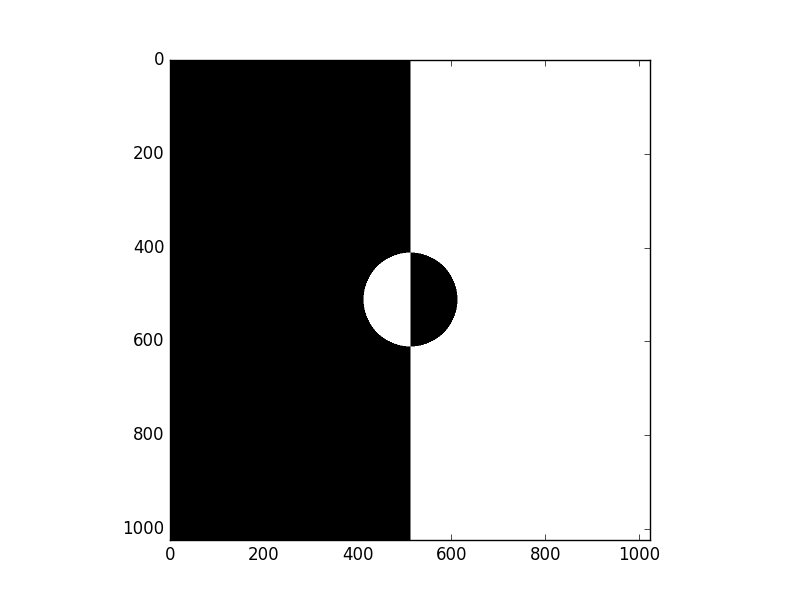
\includegraphics[width=8cm]{figure_1.png}
      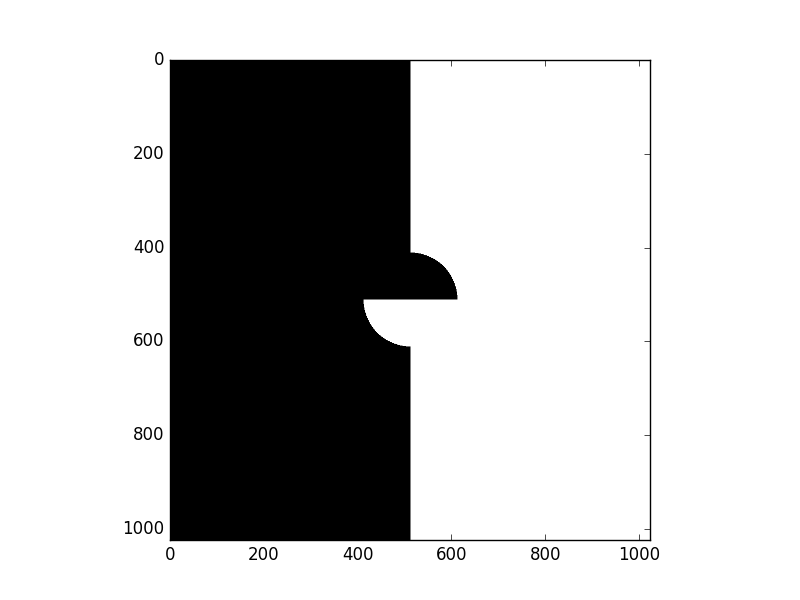
\includegraphics[width=8cm]{figure_2.png}

    \newpage

    %---------------------PROBLEM 4---------------------------------------------

    \section{Problem No.4}
      In our dataset we also have the number of likes and retweets for every message.\\
      This can give us some insight about the tweet popularity.\\
      Hence we can compute some sort of rating.\\
      The popularity of nouns is computed by the following formula:\\
      \colorbox{black!10!white}{\textbf{frequency * (1.4 + normRetweet) * (1.2 + normLikes)}}\\
      The values normRetweet and normLikes are the normalized values of retweets
      and likes for every word.\\
      To compute the number of likes and retweets for every word you just
      cumulatively collect the numbers from every tweet that the word was mentioned.

    \subsection{Solution}
      To compute the popularity of nouns, we choose the same strategy as in the
      problem No.2, except that now, we also have to know the number of likes
      and retweets the words have in every tweet.\\
      But, there is always a "but" there, if a word is repeated in a tweet, we
      have to eliminate the unnecessary summing of the same number of likes
      and retweets.\\
      After using the formula above, we see the following output:\\

      \begin{table}[H]
        \centering
        \textbf{Most popular nouns:}\\
          \begin{tabular}{l|c|r}
            \hline
            Nr & Noun & Popularity \\ \hline
            1 & i & 1064026943609 \\ \hline
            2 & time & 20386008819 \\ \hline
            3 & thing & 4889231141 \\ \hline
            4 & work & 741516848 \\ \hline
            5 & way & 640161507 \\ \hline
            6 & one & 579174359 \\ \hline
            7 & like & 535721587 \\ \hline
            8 & do & 451118807 \\ \hline
            9 & lot & 407723311 \\ \hline
            10 & internet & 358239580 \\
        \end{tabular}
      \end{table}

      Again, we notice the most favorite word of all humanity:\\
      \centerline{\emph{\textbf{I}}}\\
      But also, we observe some strange things, looks like the 7-th and 8-th\\
      words don't really look like nouns, they're verbs.\\
      That is a strange behaviour of the function \underline{pos\_tag},
      since it's responsible for tagging them as nouns.\\

    \newpage

    %-------------------PROBLEM 5-----------------------------------------------

    \section{Problem No.5}
      Write a program that receives as input an uncompleted word and prints 3
      word suggestions, followed by their frequency.\\
      The suggestions should be based on the initial dataset and sorted by the
      word frequency, computed in the first problem.\\
      The input can be any uncompleted word.\\
      Ex. Input: \colorbox{black!10!white}{app}, Output: \colorbox{black!10!white}{application (324), apple (164), appreciate (53).}\\
      Where \colorbox{black!10!white}{application} has the highest frequency, apple the second highest etc.\\
      Ex. Input: \colorbox{black!10!white}{pro}, Output: \colorbox{black!10!white}{programming (196), product (176), program (103).}\\
      Again \colorbox{black!10!white}{programming} has the highest frequency.\\

      \vspace{2em}

    \subsection{Solution}
      In this problem, we have to find the words that begin with the entered
      combination - the input.\\
      As in the previous problems, we find the frequency of each word and then,
      after finding the words that start with the input, we find the frequency
      of each one, and print only the first 3 most used words.

      \vspace{1em}

      \centerline{\textbf{Examples:}}

      \vspace{2em}

        \begin{tabular}{cc}
          \begin{minipage}{.5\linewidth}
            \hspace{4em}Input: \emph{\underline{ju}}\\
            \begin{tabular}{l|l|l}
              Nr & Word & Frequency \\ \hline
              1 & just & 159 \\ \hline
              2 & just & 3 \\ \hline
              3 & june & 3 \\
            \end{tabular}
          \end{minipage} &

          \begin{minipage}{.5\linewidth}
            \hspace{4em}Input: \emph{\underline{lo}}\\
            \begin{tabular}{l|l|l}
              Nr & Word & Frequency \\ \hline
              1 & looks & 40 \\ \hline
              2 & look & 35 \\ \hline
              3 & lot & 34 \\
            \end{tabular}
          \end{minipage}
        \end{tabular}

        \vspace{2em}

        \begin{tabular}{cc}
          \begin{minipage}{.5\linewidth}
            \hspace{4em}Input: \emph{\underline{ap}}\\
            \begin{tabular}{l|l|l}
              Nr & Word & Frequency \\ \hline
              1 & apple & 27 \\ \hline
              2 & app & 21 \\ \hline
              3 & apps & 14 \\
            \end{tabular}
          \end{minipage} &

          \begin{minipage}{.5\linewidth}
            \hspace{4em}Input: \emph{\underline{su}}\\
            \begin{tabular}{l|l|l}
              Nr & Word & Frequency \\ \hline
              1 & super & 49 \\ \hline
              2 & sure & 45 \\ \hline
              3 & support & 17 \\
            \end{tabular}
          \end{minipage}
        \end{tabular}

    \newpage

    %------------------PROBLEM 6------------------------------------------------

    \section{Bonus}
      Write a program that receives as input a word and prints 3 word suggestions,\\
      followed by the suggestion occurrences.\\
      The suggestions should be selected in the following way.\\
      You have to go through your tweets dataset and identify every occurrence
      of the input word.\\
      At every occurrence collect the word that follows the input word.\\
      That is the suggestion you are looking for.\\
      The input can be any completed word.\\
      Ex. Input: \colorbox{black!10!white}{love}, Output: \colorbox{black!10!white}{programming (5), cars (2), beer (2)}\\
      Ex. Input: \colorbox{black!10!white}{awesome}, Output: \colorbox{black!10!white}{party (10), language (4), framework (2)}

    \vspace{4em}


    \subsection{Solution}
      This problem is similar to the previous one, except that we have to find the
      occurences of the words that follow the input word and count them.\\
      The steps are pretty much the same, so let's head straight
      to the output.

      \vspace{1em}

      \centerline{\textbf{Examples:}}

      \vspace{2em}

        \begin{tabular}{cc}
          \begin{minipage}{.5\linewidth}
            \hspace{4em}Input: \emph{\underline{the}}\\
            \begin{tabular}{l|l|l}
              Nr & Word & Frequency \\ \hline
              1 & best & 30 \\ \hline
              2 & first & 18 \\ \hline
              3 & same & 18 \\
            \end{tabular}
          \end{minipage} &

          \begin{minipage}{.5\linewidth}
            \hspace{4em}Input: \emph{\underline{I}}\\
            \begin{tabular}{l|l|l}
              Nr & Word & Frequency \\ \hline
              1 & am & 75 \\ \hline
              2 & don\textquotesingle t & 54 \\ \hline
              3 & have & 53 \\
            \end{tabular}
          \end{minipage}
        \end{tabular}

        \vspace{2em}

        \begin{tabular}{cc}
          \begin{minipage}{.5\linewidth}
            \hspace{4em}Input: \emph{\underline{no}}\\
            \begin{tabular}{l|l|l}
              Nr & Word & Frequency \\ \hline
              1 & idea & 7 \\ \hline
              2 & longer & 4 \\ \hline
              3 & matter & 3 \\
            \end{tabular}
          \end{minipage} &

          \begin{minipage}{.5\linewidth}
            \hspace{4em}Input: \emph{\underline{Trump}}\\
            \begin{tabular}{l|l|l}
              Nr & Word & Frequency \\ \hline
              1 & presidency & 2 \\ \hline
              2 & is & 2 \\ \hline
              3 & will & 1 \\
            \end{tabular}
          \end{minipage}
        \end{tabular}

\end{document}
